\documentclass[12pt,a4paper]{book}

% --------------------------------------------------
% Idioma e tipografia
% --------------------------------------------------
\usepackage[brazilian]{babel}

\usepackage{fontspec}
\usepackage{unicode-math}

\setmainfont{TeX Gyre Termes}
\setsansfont{TeX Gyre Heros}
\setmathfont{TeX Gyre Termes Math}

% --------------------------------------------------
% Geometria da página
% --------------------------------------------------

\usepackage[
  top=2.5cm,
  bottom=2.5cm,
  left=2.5cm,
  right=2.5cm
]{geometry}

\usepackage{pdfpages}
\usepackage{microtype}

% --------------------------------------------------
% Espaçamento e listas
% --------------------------------------------------

\usepackage{setspace}
\onehalfspacing

\usepackage{enumitem}
\setlist{
  itemsep=2pt,
  topsep=4pt,
  parsep=0pt,
  partopsep=0pt
}

% --------------------------------------------------
% Matemática e símbolos
% --------------------------------------------------

\usepackage{amsmath}
\usepackage{xfrac}

% --------------------------------------------------
% Tabelas
% --------------------------------------------------

\usepackage{booktabs}
\usepackage{xltabular}
\usepackage{caption}

% --------------------------------------------------
% Gráficos, cores e código
% --------------------------------------------------

\usepackage{graphicx}
\usepackage{xcolor}
\usepackage{minted}

\usepackage[most]{tcolorbox}
\tcbuselibrary{minted}

% --------------------------------------------------
% Paleta de cores
% --------------------------------------------------

\definecolor{myRed}{RGB}{178,94,58}
\definecolor{myBlue}{RGB}{45,95,120}
\definecolor{myGreen}{RGB}{70,105,75}
\definecolor{myGrey}{RGB}{55,60,70}

% --------------------------------------------------
% Configuração geral das caixas
% --------------------------------------------------

\tcbset{
    enhanced,
    breakable,
    boxrule=0.8pt,
    before skip=12pt,
    after skip=14pt,
    left=10pt,
    right=10pt,
    top=7pt,
    bottom=7pt,
    fonttitle=\sffamily\bfseries,
}

% --------------------------------------------------
% Caixas
% --------------------------------------------------

\newtcolorbox{definition}[1][Definição]{
    arc=9pt,
    outer arc=10pt,
    colframe=myBlue,
    colback=myBlue!5,
    boxrule=1pt,
    title={#1},
}

\newtcolorbox{deepdive}[1][]{
    boxrule=0pt,
    frame hidden,
    sharp corners,
    borderline west={3pt}{0pt}{myGreen},
    colback=myGreen!5,
    title={#1},
    fonttitle=\sffamily\bfseries,
    attach boxed title to top left={yshift=-2mm, xshift=4mm},
    boxed title style={
        frame hidden,
        colback=myGreen!5,
    },
}

\newtcolorbox{error}[1][]{
    boxrule=0pt,
    frame hidden,
    sharp corners,
    borderline west={3pt}{0pt}{myRed},
    colback=myRed!5,
    title={#1},
    fonttitle=\sffamily\bfseries,
    attach boxed title to top left={yshift=-2mm, xshift=4mm},
    boxed title style={
        frame hidden,
        colback=myRed!5,
    },
}

% --------------------------------------------------
% Código
% --------------------------------------------------

\newtcblisting{code}[1][Código]{
    listing engine=minted,
    minted language=R,
    listing only,
    sharp corners,
    colback=myGrey!3,
    colframe=myGrey,
    boxrule=0.5pt,
    title={#1},
    minted options={
        linenos,
        numbersep=8pt,
        breaklines,
        autogobble,
        fontsize=\small,
        tabsize=20
    }
}


% --------------------------------------------------
% Títulos
% --------------------------------------------------

\usepackage{titlesec}

\titleformat{\chapter}[hang]
  {\normalfont\sffamily\huge\bfseries}
  {\textcolor{myBlue}{\thechapter}}
  {0.75em}
  {}

\titleformat{\section}[hang]
  {\normalfont\sffamily\Large\bfseries}
  {\textcolor{myBlue}{\thesection}}
  {0.6em}
  {}

\titleformat{\subsection}[hang]
  {\normalfont\sffamily\large\bfseries}
  {\textcolor{myBlue}{\thesubsection}}
  {0.5em}
  {}

\newcommand{\boxtitle}[1]{%
  {\sffamily\bfseries #1}\par
}

% --------------------------------------------------
% Cabeçalhos e rodapés
% --------------------------------------------------

\usepackage{fancyhdr}

\pagestyle{fancy}
\fancyhf{}

% Even pages
\fancyhead[LE]{\footnotesize\textit{Bioestatística para apressados}}

% Odd pages
\fancyhead[RO]{\footnotesize\leftmark}

% Page numbers
\fancyhead[RE]{\footnotesize\thepage}
\fancyhead[LO]{\footnotesize\thepage}

\renewcommand{\headrulewidth}{0.4pt}
\renewcommand{\footrulewidth}{0pt}

\setlength{\headheight}{14.5pt}

% --------------------------------------------------
% Epígrafe
% --------------------------------------------------

\usepackage{epigraph}

% --------------------------------------------------
% Hyperlinks
% --------------------------------------------------

\usepackage{hyperref}
\hypersetup{
    colorlinks=true,
    linkcolor=myBlue,
    citecolor=myGreen!70!black,
    urlcolor=myRed,
}

% --------------------------------------------------
% Document
% -------------------------------------------------
\begin{document}

\frontmatter

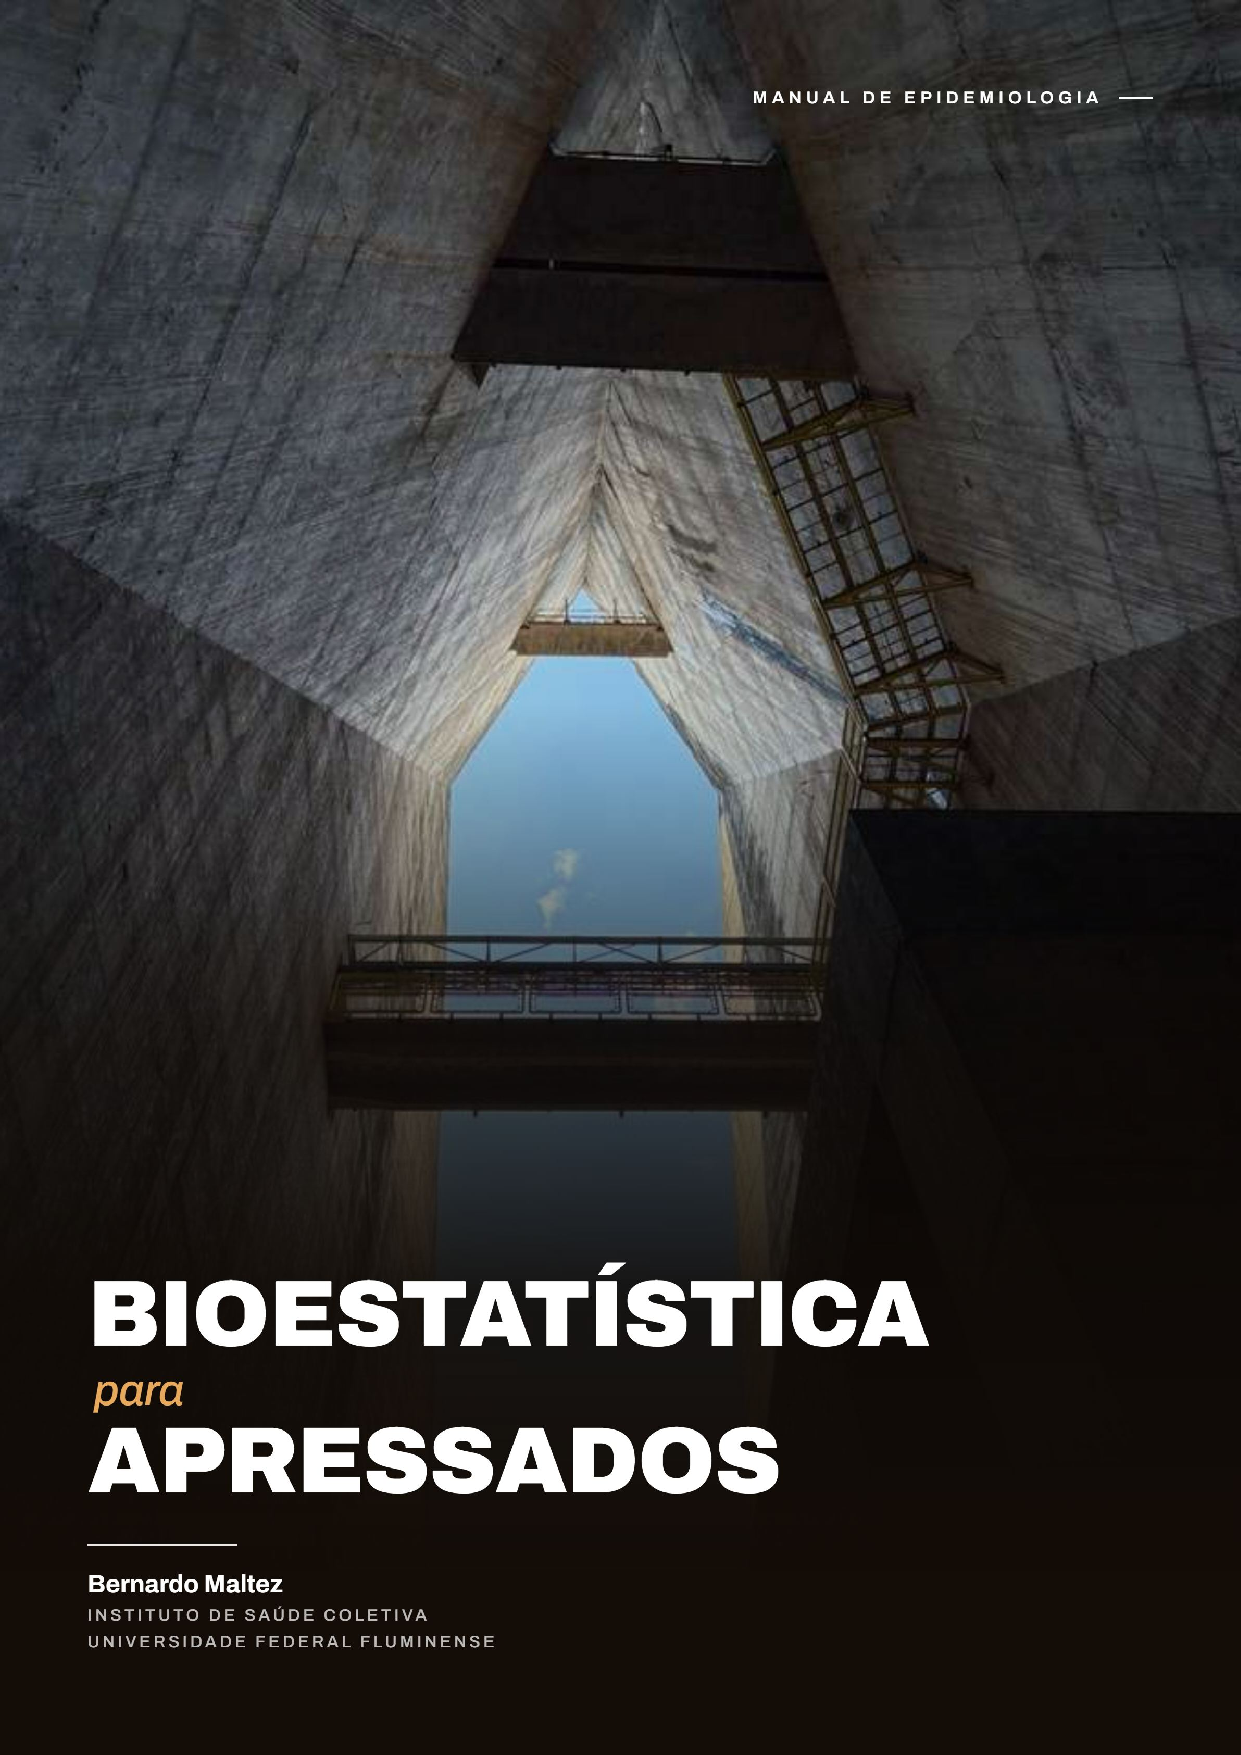
\includepdf[
    pages=1,
    fitpaper=true
]{img/cover_pt.pdf}

% --------------------------------------------------
% Epígrafe
% --------------------------------------------------

\thispagestyle{empty}

\vspace*{\fill}

\epigraph{
    ``It doesn't matter how beautiful your theory is, it doesn't matter how smart you are. If it doesn't agree with experiment, it's wrong.''
}{
    Richard P. Feynman
}

\vspace*{\fill}

% --------------------------------------------------
% Agradecimentos
% --------------------------------------------------

\chapter*{Agradecimentos}

Agradeço à minha família, aos meus amigos e a todos aqueles quecontribuíram para o desenvolvimento da estatística. Este manual só foi possível graças ao conhecimento construído ao longo dos séculos.

Agradeço especialmente aos professores Aline Silva, Felipe Guimarães e Valéria Baltar, por todo o apoio, incentivo e contribuição durante a elaboração deste material. Seus ensinamentos e sua generosidade foram fundamentais para que este projeto pudesse se concretizar.

% --------------------------------------------------
% Sumário
% --------------------------------------------------

\tableofcontents

% --------------------------------------------------
% Corpo do livro
% --------------------------------------------------

\mainmatter

\chapter*{Introdução}

A estatística é uma das ferramentas mais importantes da ciência, pois nos permite quantificar a incerteza associada aos dados e avaliar a força das evidências diante de determinado achado. Curiosamente, é comum que estudantes de estatística se limitem a memorizar fórmulas, sem de fato compreender por que as utilizam ou como devem aplicá-las na prática.

Diante desse problema, resolvi fazer meu projeto da disciplina de Epidemiologia I (Faculdade de Medicina da Universidade Federal Fluminense, Niterói, RJ) ser um pequeno manual para preencher essa lacuna. O objetivo não é realizar uma revisão completa da matéria, tampouco explicar minuciosamente como o código em R funciona, pois já existem excelentes materiais para ambas as finalidades. Este texto pretende construir uma ponte entre a teoria da bioestatística, sua aplicação prática e sua implementação no R. Por isso, privilegia-se o entendimento intuitivo da estatística em relação ao formalismo matemático.

O objetivo deste pequeno livro é auxiliar futuros pesquisadores que já possuam alguma familiaridade com a bioestatística. Não pretende ser um livro introdutório nem uma obra de referência para estatísticos experientes. A proposta é mais modesta: ajudar o leitor a compreender não apenas \textit{o que} fazer diante de um conjunto de dados, mas principalmente \textit{por que} fazê-lo e \textit{como} interpretar os resultados.

A didática e organização desta obra tem como principais referências \href{https://venhance.github.io/napkin/Napkin.pdf}{An Infinitely Large Napkin}, \href{https://mml-book.github.io/book/mml-book.pdf}{Mathematics for machine learning} e \textit{Astrofísica para apressados}, a qual o título desse manual homenageia. A capa é uma fotografia do autor da Usina Hidrelétrica de Itaipu, que visa representar como o engenho humano é capaz de lidar com grandes quantidades de água (e de dados).

\section*{Elementos Visuais: O Significado das Caixas Coloridas}

Ao longo do manual, você encontrará caixas coloridas que indicam diferentes tipos de conteúdo:

\begin{definition}
Contém definições formais, termos-chave e conceitos fundamentais. Use estas caixas como referência rápida.
\end{definition}

\begin{error}
\boxtitle{Erro}
Identifica pegadinhas, confusões típicas e interpretações equivocadas frequentes. Aprender o que \textbf{não} fazer é tão importante quanto aprender o que fazer.
\end{error}

\begin{deepdive}
\boxtitle{Aprofundamento}
Contém tópicos mais avançados, deduções matemáticas ou extensões que vão além da ementa básica. Pode ser pulado em uma primeira leitura.
\end{deepdive}

\begin{code}[Código em R]
Blocos de código comentado em linguagem R que você pode copiar, colar e executar.
\end{code}

\section*{O Artigo Utilizado Como Referência}

\begin{definition}[FIRE AND ICE: Ensaio Clínico Randomizado]
\begin{itemize}
\item \textbf{Título completo:} Cryoballoon or Radiofrequency Ablation for Paroxysmal Atrial Fibrillation

\item \textbf{Tipo de estudo:} Ensaio clínico randomizado de não inferioridade, com 762 pacientes

\item \textbf{Pergunta de pesquisa:} A crioablação é comparável (não inferior) à radioablação no tratamento da fibrilação atrial refratária a drogas?

\item \textbf{Identificador:} DOI 10.1056/NEJMoa1602014

\item \textbf{Por que foi escolhido:} Demonstra praticamente todos os conceitos abordados neste livro em um desenho real, complexo e moderno, incluindo o conceito de não inferioridade. Exemplifica amostragem, testes de hipótese, interpretação de resultados e comunicação responsável das evidências.


\end{itemize}
\end{definition}

\section*{Quero contribuir ao projeto}

Que bom! Este livro é inteiramente escrito em \LaTeX\ e desenvolvido de forma aberta. Todo o código-fonte, incluindo os capítulos, figuras, referências e demais arquivos necessários para sua compilação, está disponível no \href{https://github.com/brpmaltez/bph_book}{GitHub}.

O livro e seus demais materiais autorais são distribuídos sob a licença \textbf{Creative Commons Attribution-NonCommercial-ShareAlike 4.0 International (CC BY-NC-SA 4.0)}. Isso significa que você é livre para compartilhar, copiar e adaptar o material para fins não comerciais, desde que atribua os devidos créditos ao autor e distribua eventuais versões modificadas sob a mesma licença.

O código em \LaTeX\ e em R que acompanha o livro, por sua vez, são disponibilizados sob a \textbf{GNU GPLv3}, permitindo seu uso, modificação e redistribuição, inclusive para fins comerciais, desde que os termos da licença sejam respeitados.

Acredito que o conhecimento científico se beneficia quando pode ser compartilhado, reproduzido e aprimorado. Por isso, este projeto é desenvolvido de forma aberta: se você encontrar um erro, tiver uma sugestão ou quiser contribuir com uma melhoria, sinta-se à vontade para fazê-lo por meio do \href{https://github.com/brpmaltez/bph_book}{GitHub}.
\chapter{Amostragem}

\section{Provocação: Por que 762 pacientes e não 100?}

Abra o artigo \textbf{FIRE AND ICE} na seção \textit{"Statistical Analysis"} (dentro de \textit{Methods}) e procure por \textit{"sample size"}:

\begin{quote}
\small\itshape
"Assuming event-free 1-year survival rates of 70\% in both groups and with a noninferiority margin of 10\% (corresponding to a hazard ratio of 1.43), we calculated that 249 primary-end-point events would be required for the trial to have 80\% power to test the noninferiority of cryoballoon ablation to radiofrequency ablation, at a one-sided alpha level of 0.025. A sample size of 549 patients was originally estimated. A prespecified blinded sample-size reestimation was performed before enrollment was fully complete. On the basis of the reestimation, we calculated that 768 patients would have to be enrolled to ensure that 249 primary-end-point events would be observed."
\end{quote}

Os pesquisadores não escolheram o número de participantes simplesmente porque esse número ``parecia suficiente''. Antes do início do estudo, foi necessário estimar quantos pacientes seriam necessários para que o estudo tivesse precisão e poder estatístico adequados.

Essa é uma das primeiras ideias importantes deste capítulo:

\begin{quote}
\textit{O tamanho de uma amostra não é apenas uma questão de logística. Ele determina quanta informação conseguimos extrair dos dados.}
\end{quote}

Se estudássemos apenas 10 pacientes, poderíamos obter uma estimativa muito diferente daquela obtida ao estudar 1000 pacientes. Mas por quê?

A resposta começa com um fato aparentemente banal: \textbf{amostras diferentes produzem resultados diferentes}.

\section{Amostras e a variabilidade}

Amostras são subgrupos de uma população escolhidos segundo \textbf{determinados critérios}, que nos permitem chegar a \textbf{certas conclusões} com \textbf{alguma confiança}. Preste atenção na palavra confiança, pois ela é o ponto central de nossa discussão
Uma \textbf{população} é o conjunto de indivíduos sobre os quais queremos tirar conclusões. Uma \textbf{amostra} é um subconjunto dessa população que efetivamente observamos.

Em pesquisa clínica, quase nunca conseguimos estudar toda a população de interesse. Se quisermos conhecer a pressão arterial média de todos os adultos de uma determinada população, por exemplo, seria impraticável medir cada indivíduo. Em vez disso, selecionamos uma amostra e utilizamos seus resultados para fazer inferências sobre a população.

Mas existe um problema: \textbf{qualquer amostra é apenas uma das muitas amostras possíveis}.

\subsection{Variabilidade amostral}

\begin{definition}[Variabilidade Amostral]
Variabilidade amostral é a variação natural dos resultados obtidos quando diferentes amostras são selecionadas da mesma população.
\end{definition}

Exemplos:
\begin{itemize}
    \item Se tiramos média de pressão arterial em 10 pacientes: resultado pode ser 134.2 mmHg
    \item Se repetimos com outros 10 pacientes: resultado pode ser 136.8 mmHg
    \item A diferença de 2.6 mmHg é devido ao acaso (variabilidade amostral)
\end{itemize}

\begin{error}
\boxtitle{Variabilidade amostral não é erro de medição}
É importante distinguir \textbf{variabilidade amostral} de \textbf{erro de medição}.

A variabilidade amostral ocorre mesmo quando todas as medições são realizadas perfeitamente. Ela existe porque selecionamos apenas uma parte da população.

Já um aparelho mal calibrado, uma balança defeituosa ou uma técnica inadequada de aferição podem introduzir erros de mensuração.

\end{error}

A pergunta passa então a ser:

\begin{quote}
\textit{Se diferentes amostras produzem diferentes resultados, quão variável é a estimativa que obtivemos?}
\end{quote}

É aqui que entra a distribuição amostral.

\subsection{Distribuição Amostral}
\begin{definition}[Distribuição Amostral da Média]
Distribuição dos valores de uma estatística obtidos em várias amostras da mesma população.
\end{definition}

Se coletássemos muitas amostras (ex: 1000 amostras de n=30 cada) da mesma população, calcularíamos a média em cada amostra. Essas 1000 médias formariam uma distribuição própria, chamada \textbf{distribuição amostral}.


\begin{deepdive}
\boxtitle{O erro-padrão não é o desvio-padrão}

Essa distinção é fundamental.

O \textbf{desvio-padrão} descreve a variabilidade dos indivíduos dentro de uma população ou amostra.

O \textbf{erro-padrão} descreve a variabilidade de uma estatística, como a média, entre diferentes amostras.

Uma população pode ter indivíduos muito diferentes entre si e, ainda assim, uma média estimada com grande precisão quando o tamanho amostral é suficientemente grande.

\end{deepdive}

\begin{deepdive}

\boxtitle{Teorema Central do Limite (TCL)}

\begin{definition}[Teorema Central do Limite]
Sob condições apropriadas, à medida que o tamanho da amostra aumenta, a distribuição da média amostral aproxima-se de uma distribuição Normal, independentemente da forma da distribuição original da população.
\end{definition}

Isso não significa que os indivíduos da população precisam seguir uma distribuição Normal. A população pode apresentar uma distribuição:

\begin{itemize}
\item aproximadamente Normal;
\item assimétrica;
\item uniforme;
\item exponencial;
\item ou mesmo com múltiplos picos.
\end{itemize}

Ainda assim, sob condições adequadas, a distribuição das \textbf{médias amostrais} tende a ser aproximadamente Normal quando $n$ aumenta.
\end{deepdive}

\begin{error}
\boxtitle{Não existe um ``n mágico''}

É comum ouvir que ``o TCL funciona quando $n>30$''. Isso é apenas uma regra prática simplificada. Não existe um tamanho amostral universal a partir do qual a aproximação Normal passa a ser válida. A qualidade da aproximação depende também da distribuição original dos dados.

Uma população aproximadamente Normal pode produzir uma distribuição amostral muito próxima da Normal mesmo com amostras pequenas. Já uma população extremamente assimétrica ou com caudas muito pesadas pode exigir amostras consideravelmente maiores.

\end{error}

\section{Erro-padrão}

\begin{definition}[Erro-Padrão]
Medida da variabilidade esperada de uma estatística entre diferentes amostras.
\end{definition}

O erro-padrão mede a \textbf{variabilidade esperada} de um estimador amostral.


Para a média:
\begin{equation}
  \text{SE} = \frac{\sigma}{\sqrt{n}}
\end{equation}

Onde:
\begin{itemize}
    \item $\sigma$ = desvio-padrão populacional
    \item $n$ = tamanho da amostra
\end{itemize}

\textbf{Interpretação:} o erro-padrão quantifica a variabilidade
esperada da média amostral entre amostras repetidas da mesma população.

\textbf{Exemplo FIRE AND ICE:}

\begin{itemize}
    \item Pressão arterial: $\sigma \approx 18{,}5$ mmHg;
    \item Amostra: $n=376$ (RF);
    \item Erro-padrão:
    \[
        SE = \frac{18{,}5}{\sqrt{376}}
        \approx 0{,}95\text{ mmHg}.
    \]
\end{itemize}

Isso significa que, se repetíssemos o processo de amostragem muitas vezes, as médias amostrais apresentariam uma variabilidade caracterizada por um erro-padrão de aproximadamente $0{,}95$ mmHg.

\section{Quanto precisamos amostrar?}

Até aqui vimos que aumentar $n$ reduz a incerteza. Mas isso imediatamente produz uma nova pergunta: Quanto é suficiente?

A resposta depende da pergunta que queremos responder. Não existe uma única ``fórmula do tamanho amostral''. O cálculo depende do desenho do estudo e do objetivo da análise. Por exemplo, podemos querer:

\begin{enumerate}
\item estimar uma média com determinada precisão;
\item estimar uma proporção com determinada margem de erro;
\item detectar uma diferença entre dois grupos;
\item avaliar um desfecho de tempo até evento;
\item estimar a frequência de um evento raro.
\end{enumerate}

Cada uma dessas situações possui métodos próprios. Abaixo, iremos comentar algumas fórmulas clássicas para o cálculo do tamanho da amostra.

\subsection{Estimativa de Médias:}
\begin{equation}
  n = \frac{\sigma^2 \cdot Z_{\gamma}^2}{\epsilon^2} \quad \text{(Variância Conhecida)} 
\end{equation}

\begin{equation}
  n = \frac{s^2 \cdot t_{(n-1,\, \gamma)}^2}{\epsilon^2} \quad \text{(Variância Desconhecida)}
\end{equation}

\begin{deepdive}
\boxtitle{A distribuição t-Student e iteratividade}
O uso do valor $t$ em vez de $Z$ é uma medida de segurança. Como a distribuição $t$-Student tem caudas mais largas, ela assume que há mais incerteza quando trabalhamos com desvios padrão estimados ($s$) em vez de parâmetros reais ($\sigma$). Conforme o $n$ planejado aumenta, o valor de $t$ converge para o de $Z$ e a diferença entre as fórmulas desaparece.

Como $t$ depende dos graus de liberdade, que por sua vez dependem de $n$, o tamanho da amostra não pode ser obtido diretamente por uma única substituição. Na prática, utiliza-se um valor inicial para $n$, calcula-se o valor crítico de $t$, atualiza-se $n$ e repete-se o procedimento até que o resultado se estabilize.
\end{deepdive}

\subsection{Estimativa de Proporções:}
\begin{equation}
  n = \frac{Z_{\gamma}^2 \cdot p(1-p)}{\epsilon^2} \quad \text{(Proporção Estimada)} \qquad
\end{equation}

\begin{equation}
\qquad n = \frac{Z_{\gamma}^2}{4\epsilon^2} \quad \text{(Cenário Conservador)}
\end{equation}

\subsection{Exemplo em R}

Imagine que queremos estimar a proporção de estudantes que praticam atividade física regularmente. Desejamos um intervalo de confiança de 95\% e uma margem de erro de, no máximo, 5 pontos percentuais.

Quando não temos uma estimativa prévia da proporção, utilizamos o cenário conservador, $p=0{,}5$:

\begin{equation}
    n =
    \frac{
        z_{1-\alpha/2}^{\,2}p(1-p)
    }{
        \epsilon^2
    }.
\end{equation}

Para um intervalo de confiança de 95\%:

\[
    z_{1-\alpha/2} \approx 1{,}96.
\]

Como não conhecemos previamente $p$:

\[
    p(1-p)
    =
    0{,}5(1-0{,}5)
    =
    0{,}25.
\]

Assim:

\[
    n =
    \frac{
        1{,}96^2 \times 0{,}25
    }{
        0{,}05^2
    }
    \approx
    384{,}16.
\]

Como não podemos estudar uma fração de participante, arredondamos para cima:

\[
    \boxed{n=385}.
\]

Podemos obter o mesmo resultado diretamente no R:

\begin{code}[Código em R: Tamanho da amostra]
# Parâmetros
confianca <- 0.95
margem_erro <- 0.05
p <- 0.5

# Quantil da distribuição Normal
z <- qnorm(1 - (1 - confianca) / 2)

# Tamanho da amostra
n <- z^2 * p * (1 - p) / margem_erro^2

# Arredondar para cima
n <- ceiling(n)

cat("Tamanho da amostra:", n, "\n")
\end{code}

O resultado será:

\begin{code}[Resultado]
Tamanho da amostra: 385
\end{code}

Esse pequeno exemplo ilustra uma ideia importante do R: as funções estatísticas não substituem o raciocínio estatístico. Primeiro definimos o que queremos estimar, qual precisão desejamos e quais premissas estamos adotando. Só então transformamos esse raciocínio em código.

\begin{deepdive}
\boxtitle{E se quisermos mais precisão?}

A margem de erro aparece no denominador da fórmula:

\begin{equation}
    n \propto \frac{1}{\epsilon^2}.
\end{equation}

Portanto, reduzir a margem de erro exige um aumento considerável no tamanho da amostra.

Por exemplo, se quisermos uma margem de erro de apenas 2 pontos percentuais:

\[
    n =
    \frac{
        1{,}96^2 \times 0{,}25
    }{
        0{,}02^2
    }
    \approx
    2401.
\]

Ou seja, reduzir a margem de erro de 5\% para 2\% exige aumentar a amostra de aproximadamente 385 para 2401 indivíduos.
\end{deepdive}

\begin{error}
\boxtitle{Tamanho da amostra não é poder estatístic}

O cálculo acima responde a uma pergunta específica:

\begin{center}
\textit{Quantos indivíduos precisamos para estimar uma proporção com determinada precisão?}
\end{center}

Isso é diferente de perguntar se um estudo terá capacidade suficiente para detectar uma diferença entre grupos.

A segunda pergunta envolve o conceito de \textbf{poder estatístico}, que será discutido posteriormente.
\end{error}

\section{Intervalo de confiança}
Até agora, pensamos exclusivamente no tamanho da amostra para certo nível de certeza. Mas como isso reverbera nos resultados a serem apresentados? Vimos que as estatísticas amostrais são estimativas pontuais e estão sujeitas ao erro amostral.

A resposta para esse problema é o \textbf{intervalo de confiança}. Em vez de definir um valor específico, elencamos um intervalo no qual temos razoável certeza de que o parâmetro populacional real está. Por exemplo, podemos calcular um intervalo de confiança de 95\% para a média da altura de uma população e obter o intervalo [$1{,}73\text{ m}$ e $1{,}75\text{ m}$]

\begin{definition}[Intervalo de Confiança]
Um intervalo de confiança é um intervalo calculado a partir dos dados que, sob um procedimento frequentista repetido, contém o parâmetro populacional verdadeiro em uma proporção especificada das repetições.
\end{definition}

\begin{error}
\boxtitle{Interpretação Incorreta do Intervalo de Confiança}
Afirmar que "há 95\% de probabilidade de a verdadeira média da população estar contida no intervalo $[130, 140]$" é incorreto na perspectiva frequentista. A média populacional é um valor fixo, não uma variável aleatória. O correto é afirmar que, se o estudo for repetido 100 vezes com amostras idênticas, 95 desses intervalos conterão a verdadeira média populacional.
\end{error}

\subsection{Fórmula para médias}

\begin{equation}
  IC(\mu) = \bar{X} \pm Z_{\gamma} \cdot \frac{\sigma}{\sqrt{n}} \text{(Variância conhecida)}
\end{equation}

\begin{equation}
  IC(\mu) = \bar{X} \pm t_{(n-1,\, \gamma)} \cdot \frac{s}{\sqrt{n}} \text{(Variância desconhecida)}
\end{equation}

\subsection{Fórmula para proporções}

Para uma amostra suficientemente grande, a proporção amostral $\hat{p}$ pode
ser aproximada por uma distribuição normal:

\begin{equation}
    \hat{p}
    \approx
    N\left(
        p,\,
        \frac{p(1-p)}{n}
    \right).
\end{equation}

Como o verdadeiro valor de $p$ é desconhecido, utilizamos $\hat{p}$ para
estimar sua variabilidade. Assim, o intervalo de confiança de Wald é dado por:

\begin{equation}
    IC
    =
    \hat{p}
    \pm
    Z_{\gamma}
    \sqrt{
        \frac{\hat{p}(1-\hat{p})}{n}
    }.
\end{equation}

\begin{deepdive}
\boxtitle{Por que substituir $p$ por $\hat{p}$?}

Na prática, quase nunca conhecemos o verdadeiro valor de $p$. A proporção
amostral $\hat{p}$ é nossa estimativa de $p$ e, por isso, é utilizada para
estimar a incerteza da proporção.
\end{deepdive}

\subsection{Exemplo em R}

Depois de coletarmos os dados, podemos estimar a proporção observada e quantificar a incerteza dessa estimativa por meio de um intervalo de confiança.

A seguir, calcularemos o intervalo de confiança de 95\% para a taxa de recorrência no grupo de radiofrequência do FIRE AND ICE.

\begin{code}[Código em R: Intervalo de confiança para uma proporção]
# ============================================================
# Intervalo de confiança para uma proporção
# ============================================================

# Dados do grupo RF
n_rf <- 376
eventos_rf <- round(n_rf * 0.45)

# ------------------------------------------------------------
# Intervalo de confiança de 95%
# ------------------------------------------------------------

ic_rf <- prop.test(
  x = eventos_rf,
  n = n_rf,
  conf.level = 0.95
)

# Proporção observada
taxa_rf <- eventos_rf / n_rf

# ------------------------------------------------------------
# Apresentação do resultado
# ------------------------------------------------------------

cat("=== Intervalo de Confiança de 95% ===\n\n")

cat("Grupo RF:\n")
cat("  Eventos: ", eventos_rf, "/", n_rf, "\n", sep = "")
cat("  Proporção: ", round(taxa_rf * 100, 1), "%\n", sep = "")

cat(
  "  IC 95%: [",
  round(ic_rf$conf.int[1] * 100, 1),
  "%, ",
  round(ic_rf$conf.int[2] * 100, 1),
  "%]\n",
  sep = ""
)
\end{code}

O resultado será aproximadamente:

\begin{code}[Resultado]
=== Intervalo de Confiança de 95% ===

Grupo RF:
  Eventos: 169/376
  Proporção: 44.9 %
  IC 95%: [39.9 %, 50.1 %]
\end{code}

A estimativa pontual da taxa de recorrência é, portanto, $44{,}9\%$.

O intervalo de confiança de 95\% fornece uma medida da incerteza associada a essa estimativa, resultando no intervalo $[39{,}9\%,\,50{,}1\%]$.

Observe que utilizamos \texttt{prop.test()} em vez de calcular manualmente o intervalo de Wald apresentado anteriormente. Isso ocorre porque, embora a aproximação de Wald seja útil para compreender a construção do intervalo, outros métodos apresentam propriedades melhores em diversas situações. O \texttt{prop.test()} utiliza uma abordagem baseada no teste de qui-quadrado para construir o intervalo.

\section{Resumo}

Neste capítulo, aprendemos que:

\begin{enumerate}
    \item \textbf{Amostras diferentes produzem resultados diferentes:} essa é a variabilidade amostral.
    \item \textbf{O erro-padrão mede a incerteza de uma estimativa:} para a média, ele diminui aproximadamente com $1/\sqrt{n}$.
    \item \textbf{Aumentar o tamanho da amostra aumenta a precisão:} mas o tamanho necessário depende da pergunta de pesquisa.
    \item \textbf{O intervalo de confiança quantifica a incerteza:} uma estimativa pontual isolada não conta toda a história.
    \item \textbf{Para proporções,} podemos calcular o tamanho amostral necessário para atingir determinada margem de erro.
    \item \textbf{No R,} funções como \texttt{qnorm()} e \texttt{prop.test()} permitem transformar esses conceitos em cálculos reproduzíveis.
    \item \textbf{Intervalos individuais não substituem comparações entre grupos:} para comparar grupos, devemos analisar diretamente a medida de efeito de interesse.
\end{enumerate}
\chapter{Testes de Hipótese}

No capítulo anterior, estimamos parâmetros populacionais --- uma média ou uma proporção --- e expressamos a incerteza dessa estimativa através de um intervalo de confiança. O teste de hipóteses aborda um problema relacionado, porém distinto: em vez de perguntar "qual é o valor do parâmetro?", perguntamos "os dados são compatíveis com um valor específico (ou com a ausência de um efeito) que suponho a priori?"

\section{Como pensar antes de escolher um teste}

Uma dificuldade comum no início do estudo da estatística é imaginar que cada
pergunta científica corresponde a um teste estatístico específico. Essa
abordagem transforma a estatística em uma coleção de procedimentos a serem
memorizados: teste-$t$, qui-quadrado, Fisher, ANOVA, correlação e assim por
diante.

Uma abordagem mais útil é começar pela \textbf{pergunta científica} e, a
partir dela, determinar qual método estatístico é apropriado. A escolha do
teste não deve ser feita simplesmente pelo nome da variável ou por uma regra
isolada, mas pelo conjunto de características do problema.

Uma forma de organizar esse raciocínio é:

\begin{enumerate}
\item Pergunta científica
\item Desenho do estudo
\item Tipos de variáveis e estrutura dos grupos
\item Pressupostos
\item Método estatístico
\end{enumerate}

A \textbf{pergunta científica} determina o que desejamos investigar. Podemos
querer descrever uma população, comparar grupos, investigar uma associação,
estimar um efeito ou avaliar uma hipótese causal.

O \textbf{desenho do estudo} fornece informações fundamentais para essa
escolha. Dados provenientes de um ensaio clínico randomizado, por exemplo,
possuem uma estrutura diferente daquela encontrada em um estudo observacional.
Da mesma forma, medidas repetidas no mesmo indivíduo não podem ser tratadas
como se fossem observações independentes.

Em seguida, devemos considerar o \textbf{tipo de variável} envolvida. Uma variável quantitativa, como idade ou pressão arterial, exige procedimentos diferentes daqueles utilizados para uma variável categórica, como sexo, tratamento ou ocorrência de um evento.

Também é necessário observar a \textbf{estrutura dos grupos}. Quando existem
dois grupos, por exemplo, devemos perguntar se eles são independentes ou se as observações estão pareadas. Quando existem três ou mais grupos, a estratégia de análise pode ser diferente. A mesma variável pode, portanto, ser analisada por métodos distintos dependendo da maneira como os dados foram coletados.

Por fim, devem ser avaliados os \textbf{pressupostos} do procedimento. Alguns
métodos dependem de condições relacionadas à distribuição dos dados,
independência das observações, homogeneidade das variâncias ou tamanho das
contagens esperadas. Quando essas condições não são adequadas, outro
procedimento pode ser mais apropriado.

Assim, o teste estatístico deve ser visto como a \textbf{consequência de uma
sequência de decisões}, e não como o ponto de partida da análise.

Neste capítulo, serão apresentados os principais conceitos que fundamentam os
testes de hipótese. No capítulo seguinte, esses procedimentos serão organizados de forma prática, mostrando \textbf{quando utilizar cada um} e como escolher entre alternativas possíveis diante de diferentes tipos de dados e desenhos de estudo.

\section{Associação, diferença e causalidade}

Duas variáveis estão associadas quando a distribuição de uma varia de acordo
com os valores ou categorias da outra.Por exemplo, pode existir associação entre idade e pressão arterial se os
valores de pressão arterial tenderem a ser diferentes em indivíduos de
idades diferentes.

Uma comparação entre grupos também pode ser vista como uma forma particular
de estudar associação. Ao comparar a idade entre os grupos RF e Cryo, estamos
investigando se a distribuição da idade varia de acordo com o grupo de
tratamento.

É importante, entretanto, distinguir três perguntas:

\begin{itemize}
    \item \textbf{Descrição:} quais são os valores observados nos dados?
    \item \textbf{Associação:} existe relação estatística entre as variáveis?
    \item \textbf{Causalidade:} uma variável produz mudança na outra?
\end{itemize}

Essas perguntas não são equivalentes.

Associação não implica causalidade. Uma associação observada pode decorrer de:

\begin{itemize}
    \item efeito causal;
    \item causalidade reversa;
    \item confundimento;
    \item viés de seleção;
    \item viés de mensuração;
    \item acaso.
\end{itemize}

Em um ensaio clínico randomizado, a randomização ajuda a equilibrar, em
expectativa, fatores de prognóstico entre os grupos. Quando o estudo é
adequadamente conduzido, isso fortalece a interpretação causal da diferença
entre os tratamentos.

Em um estudo observacional, entretanto, uma associação entre exposição e
desfecho não estabelece, por si só, que a exposição causou o desfecho.

\section{Hipótese Nula e Alternativa}
Todo teste de hipóteses parte de duas afirmações mutuamente excludentes sobre a população:
\begin{itemize}
    \item \textbf{Hipótese nula ($H_0$):} afirma que não há efeito, diferença ou associação --- é o estado de "nada de novo", tomado como verdadeiro até que haja evidência suficiente em contrário. Ex.: \emph{"o novo medicamento tem o mesmo efeito que o placebo"}.
    \item \textbf{Hipótese alternativa ($H_1$ ou $H_a$):} afirma exatamente o oposto --- existe efeito, diferença ou associação. Ex.: \emph{"o novo medicamento reduz a pressão arterial mais do que o placebo"}.
\end{itemize}

A lógica é semelhante à de um julgamento: presume-se a inocência ($H_0$) e só se condena (rejeita-se $H_0$) diante de evidência que torne essa hipótese muito improvável. O teste nunca "prova" $H_0$ verdadeira --- apenas indica se há ou não evidência suficiente para rejeitá-la.

\begin{error}
\boxtitle{Direcionalidade e p-hacking}
A hipótese alternativa pode ser \textbf{bilateral} ($H_1: \mu \neq \mu_0$, o efeito pode ir em qualquer direção) ou \textbf{unilateral} ($H_1: \mu > \mu_0$ ou $H_1: \mu < \mu_0$, quando só uma direção do efeito é biologicamente plausível ou relevante). A escolha deve ser feita antes de olhar os dados --- decidir isso depois de ver o resultado é uma forma de viés conhecida como \emph{p-hacking}.
\end{error}

\section{O Valor-p: Definição correta e interpretação clínica}

\begin{definition}[Definição: Valor-p]
\textbf{Valor-p:} A probabilidade de observar um resultado tão extremo quanto (ou mais extremo do que) o obtido na amostra, assumindo que a hipótese nula é verdadeira.
\end{definition}

Um valor-$p$ pequeno indica que o resultado observado seria raro se $H_0$ fosse de fato verdadeira --- o que enfraquece a credibilidade de $H_0$. Convencionalmente, compara-se o valor-$p$ a um limiar de significância ($\alpha$), geralmente $0{,}05$:
\begin{itemize}
    \item $p < \alpha$: rejeita-se $H_0$ --- resultado "estatisticamente significativo".
    \item $p \ge \alpha$: não se rejeita $H_0$ --- não há evidência suficiente para afastar a hipótese de ausência de efeito.
\end{itemize}

\begin{deepdive}
\boxtitle{Aprofundando: O que o valor-p NÃO significa}

\begin{itemize}
    \item Não é a probabilidade de $H_0$ ser verdadeira, nem de $H_1$ ser verdadeira.
    \item Não mede o tamanho ou a relevância clínica do efeito --- uma amostra muito grande pode gerar $p < 0{,}05$ para uma diferença clinicamente irrelevante (ex.: $0{,}1\text{ mmHg}$ de diferença de pressão arterial).
    \item Não é a probabilidade de o achado ser "por acaso" no sentido coloquial, e $p = 0{,}06$ não é qualitativamente diferente de $p = 0{,}04$ --- o limiar de $0{,}05$ é uma convenção, não uma lei natural.
\end{itemize}
Por isso, diretrizes editoriais recomendam reportar sempre o intervalo de confiança e uma medida de tamanho de efeito ao lado do valor-$p$.
\end{deepdive}

\section{Exemplo em R}

Suponha que, em uma população de referência, a pressão arterial sistólica
média seja de $130$ mmHg. Um pesquisador deseja investigar se pacientes
submetidos a determinado tratamento apresentam uma pressão arterial sistólica
média diferente desse valor.

Uma amostra de $100$ pacientes apresentou média de $134$ mmHg. Para simplificar
o exemplo, suponha que o desvio-padrão populacional seja conhecido e igual a
$20$ mmHg.

A pergunta científica é, portanto:

\begin{quote}
A pressão arterial sistólica média dos pacientes é diferente de
$130$ mmHg?
\end{quote}

Como a pergunta é sobre uma única média populacional e o desvio-padrão
populacional é conhecido, podemos utilizar um teste $Z$ para uma média.

\subsection{Hipóteses}

O primeiro passo é transformar a pergunta científica em hipóteses
estatísticas.

A hipótese nula representa o valor de referência:

\[
H_0:\mu=130.
\]

A hipótese alternativa representa a possibilidade de uma diferença:

\[
H_1:\mu\neq130.
\]

O teste é, portanto, \textbf{bilateral}, pois estamos interessados em detectar
uma diferença em qualquer direção.

\begin{itemize}
    \item $H_0$: a média populacional é $130$ mmHg;
    \item $H_1$: a média populacional é diferente de $130$ mmHg.
\end{itemize}

O nível de significância será definido como:

\[
\alpha=0{,}05.
\]

Isso significa que, sob as condições do teste, aceitamos uma probabilidade de
$5\%$ de cometer um erro Tipo I caso rejeitemos uma hipótese nula verdadeira.

\subsection{Calculando a estatística de teste}

Para o teste $Z$ de uma média, utilizamos:

\[
Z=
\frac{\bar{x}-\mu_0}
{\sigma/\sqrt{n}},
\]

em que $\bar{x}$ é a média observada na amostra, $\mu_0$ é o valor especificado
pela hipótese nula, $\sigma$ é o desvio-padrão populacional e $n$ é o tamanho
da amostra.

Neste exemplo:

\[
\bar{x}=134,\qquad
\mu_0=130,\qquad
\sigma=20,\qquad
n=100.
\]

Portanto:

\[
Z=
\frac{134-130}{20/\sqrt{100}}
=
\frac{4}{2}
=
2.
\]

A estatística de teste é, portanto, $Z=2$.

Podemos realizar esse cálculo diretamente em R.

\begin{code}[Código: cálculo da estatística Z]
# Média observada na amostra
media <- 134

# Valor da média especificado em H0
media_nula <- 130

# Desvio-padrão populacional conhecido
dp_populacional <- 20

# Tamanho da amostra
n <- 100

# Cálculo da estatística Z
z <- (media - media_nula) /
  (dp_populacional / sqrt(n))

z
\end{code}

Cada parte do código corresponde diretamente aos elementos da fórmula
estatística:

\begin{itemize}
    \item \texttt{media} representa a média observada, $\bar{x}$;
    \item \texttt{media\_nula} representa o valor proposto por $H_0$, $\mu_0$;
    \item \texttt{dp\_populacional} representa $\sigma$;
    \item \texttt{n} representa o tamanho da amostra;
    \item a última expressão calcula a estatística $Z$.
\end{itemize}

O resultado é:

\begin{code}[Resultado da estatística Z]
[1] 2
\end{code}

Isso significa que a média observada está a $2$ erros-padrão do valor
especificado pela hipótese nula.

\subsection{Calculando o valor-p}

Como nossa hipótese alternativa é bilateral, devemos considerar resultados extremos tanto acima quanto abaixo de
$130$ mmHg. A distribuição utilizada é a distribuição normal padrão. Em R, a função
\texttt{pnorm()} fornece probabilidades acumuladas dessa distribuição.

Podemos calcular o valor-$p$ da seguinte maneira:

\begin{code}[Código: cálculo do valor-p]
# Probabilidade de observar um valor
# pelo menos tão extremo quanto |Z| = 2
p_valor <- 2 * (1 - pnorm(abs(z)))

p_valor
\end{code}

A função \texttt{abs()} transforma $Z=2$ em seu valor absoluto. Isso é útil
porque, em um teste bilateral, estamos interessados na distância da estatística
em relação a zero, independentemente da direção.

A expressão $1-\texttt{pnorm}(|Z|)$ calcula a probabilidade de observar um valor pelo menos tão grande quanto o
valor observado em uma das caudas. Multiplicamos essa probabilidade por $2$
porque o teste é bilateral.

O resultado é aproximadamente:

\begin{code}[Resultado do valor-p]
[1] 0.0455
\end{code}

Portanto,

\[
p\approx0{,}0455.
\]

\subsection{Tomando a decisão}

Agora podemos comparar o valor-$p$ com o nível de significância definido
anteriormente:

\[
p=0{,}0455 < \alpha=0{,}05.
\]

Assim, rejeitamos $H_0$.

Podemos também fazer essa decisão diretamente no R:

\begin{code}[Código: decisão do teste]
# Nível de significância
alpha <- 0.05

# Regra de decisão
if (p_valor < alpha) {
  print("Rejeitar H0")
} else {
  print("Não rejeitar H0")
}
\end{code}

O resultado será:

\begin{code}[Resultado da decisão]
[1] "Rejeitar H0"
\end{code}

\subsection{Interpretação}

Podemos concluir que, neste exemplo, há \textbf{evidência estatística de que a
média populacional da pressão arterial sistólica seja diferente de
$130$ mmHg}.

O teste não demonstra que $H_1$ é verdadeira. Ele indica que os dados observados
seriam relativamente pouco compatíveis com $H_0$, assumindo que as condições
do teste sejam válidas. Também não podemos interpretar $p=0{,}0455$ como ``uma probabilidade de
4,55\% de $H_0$ ser verdadeira''. O valor-$p$ é calculado \textbf{assumindo
que $H_0$ é verdadeira}.

Além disso, a significância estatística não informa, por si só, se uma
diferença de $4$ mmHg é clinicamente relevante. Para essa avaliação, devemos
considerar a magnitude do efeito, sua incerteza e o contexto clínico.

\begin{error}
\boxtitle{Não rejeitar $H_0$ não significa provar que não existe efeito}

Se o valor-$p$ fosse maior que $0{,}05$, a conclusão seria ``não rejeitar
$H_0$''. Isso não significaria que a média populacional é necessariamente
igual a $130$ mmHg.

Na verdade, significaria apenas que os dados não forneceram evidência estatística
suficiente para rejeitar esse valor de referência, considerando o procedimento
e o nível de significância adotados.

Essa distinção é importante porque a capacidade de detectar uma diferença
depende, entre outros fatores, do tamanho da amostra, da variabilidade dos
dados e do tamanho do efeito. Esses fatores serão discutidos posteriormente
ao estudarmos o poder estatístico.
\end{error}

\section{Erros de Decisão}
Como toda decisão baseada em amostra, o teste de hipóteses está sujeito a erro. Existem dois tipos possíveis, resumidos na Tabela~\ref{tab:erros_decisao}.

\begin{center}
\captionof{table}{Matriz de Decisão e Tipos de Erro em Testes de Hipóteses}
\label{tab:erros_decisao}

\vspace{2mm}

\begin{tabular}{l c c}
\toprule
\textbf{Decisão do Teste} & \textbf{$H_0$ Verdadeira} & \textbf{$H_0$ Falsa} \\
\midrule
\textbf{Rejeita $H_0$} &
Erro Tipo I ($\alpha$) --- Falso Positivo &
Decisão Correta (Poder = $1-\beta$) \\

\textbf{Não rejeita $H_0$} &
Decisão Correta &
Erro Tipo II ($\beta$) --- Falso Negativo \\
\bottomrule
\end{tabular}
\end{center}

\subsection{Erro Tipo I}
Ocorre quando rejeitamos $H_0$ sendo ela, na realidade, verdadeira --- concluímos que há um efeito que de fato não existe (falso positivo). A probabilidade máxima aceita para esse erro é o próprio nível de significância $\alpha$ (tipicamente $0{,}05$, ou seja, $5\%$ de chance).

\subsection{Erro Tipo II}
Ocorre quando não rejeitamos $H_0$ sendo ela, na realidade, falsa --- deixamos de detectar um efeito que de fato existe (falso negativo). Sua probabilidade é denotada por $\beta$, e o complemento ($1-\beta$) é chamado de \textbf{poder do teste}.
\begin{error}
\boxtitle{Confundir Significância Estatística com Relevância Clínica}

Amostras excessivamente grandes aumentam o poder estatístico a ponto de produzir $p < 0{,}05$ para diferenças minúsculas (por exemplo, uma redução de $0{,}1\text{ mmHg}$ na pressão arterial) sem qualquer impacto prático no prognóstico do paciente.
\end{error}

\section{Poder estatístico}

O \textbf{poder estatístico} está diretamente relacionado ao Erro Tipo II. Se
$\beta$ é a probabilidade de não rejeitar $H_0$ quando existe um efeito de
determinado tamanho, então:

\[
\text{Poder}=1-\beta.
\]

Em outras palavras, o poder é a probabilidade de o teste \textbf{rejeitar
corretamente $H_0$ quando uma diferença ou efeito de determinado tamanho
realmente existe}.

Isso significa que o poder não é uma propriedade fixa de um teste ou de um
estudo. Ele depende do tamanho do efeito que se deseja detectar. Um estudo
pode ter alto poder para detectar uma diferença grande, mas poder muito menor
para detectar uma diferença pequena.

\begin{definition}[Poder estatístico]
\textbf{Poder estatístico:} probabilidade de rejeitar corretamente a hipótese
nula quando existe, na população, um efeito de determinado tamanho sob a
hipótese alternativa.

\[
\text{Poder}=1-\beta.
\]
\end{definition}

O poder é determinado principalmente por quatro componentes:

\begin{itemize}
    \item \textbf{tamanho da amostra ($n$):} amostras maiores geralmente
    aumentam o poder;

    \item \textbf{tamanho do efeito:} efeitos maiores são mais fáceis de
    detectar e, portanto, aumentam o poder;

    \item \textbf{nível de significância ($\alpha$):} aumentar $\alpha$
    torna mais fácil rejeitar $H_0$ e, consequentemente, aumenta o poder,
    embora também aumente a probabilidade de Erro Tipo I;

    \item \textbf{variabilidade dos dados:} quanto maior a variabilidade
    em relação ao efeito que se deseja detectar, mais difícil é identificar
    esse efeito e menor tende a ser o poder.
\end{itemize}

Podemos representar essa relação de forma simplificada como:

\[
\text{Poder}
=
f(n,\text{tamanho do efeito},\alpha,\text{variabilidade}).
\]

\subsection{Poder e tamanho da amostra}

Essa relação é particularmente importante no planejamento de estudos.

Suponha que um pesquisador queira comparar dois tratamentos e considere que
uma diferença de $5$ mmHg na pressão arterial seja clinicamente relevante.
Antes de coletar os dados, ele pode perguntar:

\begin{quote}
Quantos participantes são necessários para que o estudo tenha, por exemplo,
$90\%$ de probabilidade de detectar uma diferença de $5$ mmHg, caso ela
realmente exista?
\end{quote}

Essa é uma pergunta de \textbf{cálculo de tamanho amostral baseado em poder}.

Em um planejamento prospectivo, o pesquisador geralmente especifica:

\begin{itemize}
    \item o efeito mínimo considerado clinicamente relevante;
    \item a variabilidade esperada dos dados;
    \item o nível de significância $\alpha$;
    \item o poder desejado, frequentemente $80\%$ ou $90\%$.
\end{itemize}

A partir dessas informações, determina-se o tamanho de amostra necessário.

Por exemplo, se um estudo for planejado com poder de $90\%$, isso significa que,
\textbf{se o efeito especificado no planejamento realmente existir}, o
procedimento estatístico terá aproximadamente $90\%$ de probabilidade de
rejeitar $H_0$ nas condições assumidas.

Isso não significa que o estudo terá $90\%$ de probabilidade de encontrar
qualquer efeito que exista. Um efeito menor que aquele considerado no
planejamento pode ser muito mais difícil de detectar.

\begin{deepdive}
\boxtitle{Poder, tamanho do efeito e relevância clínica}

O conceito de poder ajuda a estabelecer uma conexão importante entre
estatística e medicina.

Considere dois estudos que utilizam o mesmo nível de significância e o mesmo
teste estatístico. O primeiro foi planejado para detectar uma diferença de
$10$ mmHg, enquanto o segundo foi planejado para detectar uma diferença de
$2$ mmHg.

Mesmo que tenham o mesmo número de participantes, o segundo estudo precisará
de uma amostra maior para alcançar o mesmo poder, pois detectar uma diferença
menor em relação à variabilidade dos dados é mais difícil.

Por isso, o tamanho amostral não deve ser escolhido apenas pela conveniência
ou pela disponibilidade de participantes. Idealmente, ele deve estar
relacionado a uma diferença que tenha significado científico ou clínico.

O conceito de \textbf{menor efeito clinicamente importante} é particularmente
útil nesse contexto: o objetivo não é simplesmente ter poder suficiente para
detectar algum efeito, mas ter poder suficiente para detectar um efeito que
seja relevante para a pergunta científica.
\end{deepdive}

\begin{error}
\boxtitle{Não confundir poder com probabilidade de o resultado ser significativo}
Um estudo com poder de $80\%$ não significa que exista uma probabilidade de
$80\%$ de obter $p<0{,}05$ independentemente do que acontecer nos dados.

O poder de $80\%$ é definido \textbf{para um determinado tamanho de efeito,
sob determinadas condições e pressupostos}. Se esse efeito realmente existir
e as demais condições do planejamento forem adequadas, a probabilidade de
rejeitar $H_0$ será aproximadamente $80\%$.

Da mesma forma, um estudo com baixo poder que produza $p\geq0{,}05$ não
permite concluir que o efeito seja inexistente. O resultado pode simplesmente
refletir uma capacidade insuficiente de detectar o efeito de interesse.
\end{error}

\begin{error}
\boxtitle{Poder pós-hoc}

O cálculo de poder é mais útil quando realizado \textbf{antes da coleta dos
dados}, durante o planejamento do estudo.

Depois que os dados já foram coletados e o resultado do teste é conhecido,
calcular um chamado ``poder observado'' com base no efeito estimado na própria
amostra geralmente acrescenta pouca informação. Esse cálculo está fortemente
relacionado ao valor-$p$ observado e pode ser enganoso como forma de explicar
um resultado não significativo.

Quando um estudo não encontra significância estatística, é mais informativo
examinar:

\begin{itemize}
    \item a estimativa do efeito;
    \item seu intervalo de confiança;
    \item a precisão da estimativa;
    \item o efeito mínimo clinicamente relevante;
    \item e, quando apropriado, o poder planejado do estudo.
\end{itemize}

Assim, a pergunta adequada não é simplesmente ``o estudo teve poder
suficiente?'', mas:

\begin{quote}
Os dados permitem excluir efeitos clinicamente relevantes com uma precisão
adequada?
\end{quote}
\end{error}

\subsection{Exemplo em R}

Quando um teste não encontra diferença significativa, surge uma pergunta
importante: será que realmente não há diferença, ou o estudo não tinha
capacidade suficiente para detectar um efeito clinicamente relevante?

\begin{code}[Cálculo prospectivo do tamanho amostral]
library(pwr)

# Diferença clinicamente relevante
diferenca <- 5

# Desvio-padrão esperado
dp <- 18

# Tamanho de efeito padronizado
d <- diferenca / dp

# Parâmetros do planejamento
alpha <- 0.05
poder_desejado <- 0.90

# Calcular tamanho de amostra por grupo
planejamento <- pwr.t.test(
  d = d,
  sig.level = alpha,
  power = poder_desejado,
  alternative = "two.sided",
  type = "two.sample"
)

planejamento
\end{code}

\begin{code}[Resultado do cálculo]
        Two-sample t test power calculation 

            n = 273.3163
            d = 0.2777778
    sig.level = 0.05
        power = 0.9
alternative = two.sided

NOTE: n is number in *each* group
\end{code}

O resultado informa o número aproximado de participantes necessários em cada
grupo para alcançar o poder especificado, dadas as demais premissas do
planejamento.

É importante perceber que o poder é definido para um \textbf{determinado
tamanho de efeito}. Um estudo pode ter alto poder para detectar uma diferença
grande e poder muito menor para detectar uma diferença pequena.

\begin{deepdive}
\boxtitle{Por que usar o cálculo baseado em poder?}

O cálculo baseado em poder é mais adequado quando o objetivo é planejar um
estudo para detectar uma \textbf{diferença clinicamente relevante}. Nesse caso, especificamos previamente o tamanho do efeito que desejamos detectar, a
variabilidade esperada, o nível de significância e o poder desejado.

A fórmula baseada na margem de erro, por outro lado, é apropriada quando o
objetivo principal é obter uma estimativa com determinada \textbf{precisão},
por exemplo, estimar uma proporção com margem de erro de $5\%$ em um intervalo
de confiança de $95\%$. Ela não considera diretamente qual diferença entre
grupos seria clinicamente importante nem a probabilidade de detectar essa
diferença.

Assim, para um estudo comparativo ou experimental, em que queremos saber
\emph{quantos participantes são necessários para detectar um efeito relevante}, o cálculo baseado em poder é geralmente a abordagem mais adequada.
\end{deepdive}


\section{Resumo}
\begin{itemize}
    \item \textbf{$H_0$ e $H_1$} representam hipóteses mutuamente excludentes
    sobre a população. A hipótese alternativa pode ser bilateral ou
    unilateral, e sua direção deve ser definida antes da análise dos dados.

    \item \textbf{O valor-$p$} quantifica a compatibilidade dos dados, ou de
    resultados ainda mais extremos, com a hipótese nula. Ele não representa a
    probabilidade de $H_0$ ser verdadeira.

    \item \textbf{Não rejeitar $H_0$ não significa provar sua verdade}.
    Ausência de evidência estatística suficiente para detectar uma diferença
    não demonstra que os grupos sejam iguais.

    \item \textbf{Erro Tipo I} ocorre quando rejeitamos uma hipótese nula
    verdadeira, enquanto o \textbf{Erro Tipo II} ocorre quando não rejeitamos
    uma hipótese nula falsa.

    \item \textbf{O poder estatístico} é a probabilidade de detectar um efeito
    de determinado tamanho quando esse efeito realmente existe. Ele depende,
    entre outros fatores, do tamanho da amostra, do tamanho do efeito e do
    nível de significância.

    \item \textbf{Significância estatística não é sinônimo de relevância
    clínica}. A interpretação de um resultado deve considerar a magnitude do
    efeito, seu intervalo de confiança e o contexto científico e clínico.

    \item \textbf{Associação não implica causalidade}. A interpretação causal
    depende do desenho do estudo e da possibilidade de controlar fontes de
    viés e confundimento.

    \item \textbf{A escolha do método estatístico começa pela pergunta
    científica}, passando pelo desenho do estudo, tipo de variável, estrutura
    dos grupos e pressupostos do procedimento.
\end{itemize}


\chapter{Quando usar cada teste?}

\section{Provocação: como comparar grupos e avaliar relações entre variáveis?}

No estudo FIRE AND ICE, os pesquisadores compararam duas técnicas de ablação
para fibrilação atrial: crioablação por balão e ablação por radiofrequência.
A pergunta principal do estudo era se as duas estratégias apresentavam eficácia
comparável dentro de uma margem de não inferioridade previamente definida.

Além do desfecho principal, os dados permitem formular perguntas estatísticas
mais simples e fundamentais:

\begin{itemize}
    \item A idade dos participantes é semelhante nos dois grupos?
    \item A proporção de homens difere entre os grupos?
    \item O tempo médio de procedimento difere entre os tratamentos?
    \item Existe associação entre idade e pressão arterial?
    \item Existe associação entre o grupo de tratamento e uma complicação?
    \item Como comparar três ou mais grupos quando a variável de interesse é quantitativa?
\end{itemize}

Essas perguntas envolvem principalmente duas ideias:

\begin{itemize}
    \item \textbf{comparação:} investigar se uma variável apresenta valores ou
    distribuições diferentes entre grupos;
    \item \textbf{associação:} investigar se os valores ou categorias de uma
    variável estão relacionados aos de outra.
\end{itemize}

Um resultado estatisticamente não significativo não demonstra que não exista
qualquer diferença ou associação. Significa que, sob o modelo e as hipóteses
adotados, os dados não forneceram evidência estatística suficiente para
rejeitar a hipótese nula.

Da mesma forma, um resultado estatisticamente significativo não informa, por
si só, se o efeito é grande, clinicamente importante ou causal.

\section{Testes para uma média}

Quando existe uma única amostra e a pergunta é comparar sua média com um valor
de referência, podemos utilizar um teste para uma média.

\subsection{Teste-t de uma amostra}

O teste-$t$ de uma amostra é apropriado quando queremos avaliar se a média
populacional difere de um valor de referência $\mu_0$, especialmente quando
o desvio-padrão populacional é desconhecido.

As hipóteses, em um teste bilateral, são:

\begin{itemize}
    \item $H_0:\mu=\mu_0$;
    \item $H_1:\mu\neq\mu_0$.
\end{itemize}

A estatística de teste é:

\begin{equation}
  t= \frac{\bar X-\mu_0}{s/\sqrt{n}}
\end{equation}

com:

\begin{equation}
  gl=n-1.
\end{equation}

O teste pressupõe, principalmente, independência das observações e, em
amostras pequenas, distribuição aproximadamente normal da variável na
população. Em amostras maiores, o teste pode ser bastante robusto a desvios
moderados da normalidade, embora valores extremos e forte assimetria ainda
possam ser problemáticos.

Em R, o procedimento pode ser realizado com:

\begin{code}[Código: teste-$t$ de uma amostra]
resultado_t1 <-
  t.test(
    x = dados$pressao,
    mu = 120,
    alternative = "two.sided"
  )

resultado_t1
\end{code}

O intervalo de confiança da média fornece informação complementar ao
valor-$p$ e deve ser considerado na interpretação.

\subsection{Teste-z para uma média}

O teste-$z$ para uma média utiliza a distribuição normal padrão e pressupõe
que o desvio-padrão populacional $\sigma$ seja conhecido:

\begin{equation}
  z= \frac{\bar X-\mu_0}{\sigma/\sqrt{n}}.
\end{equation}

Na prática, essa situação é relativamente incomum em aplicações biomédicas.
Quando $\sigma$ é desconhecido e precisa ser estimado pela amostra, o
teste-$t$ é geralmente o procedimento apropriado.

Por isso, embora o teste-$z$ seja importante para compreender a teoria dos
testes de hipóteses, o teste-$t$ é muito mais comum na prática quando estamos
comparando uma média com um valor de referência.

\section{Comparação de duas médias}

Quando a variável de interesse é quantitativa e existem dois grupos, a
primeira pergunta a ser feita é se as observações são independentes ou
pareadas.

\subsection{Teste-t de Student pareado}

O teste-$t$ pareado é utilizado quando duas observações estão naturalmente
relacionadas.

Exemplos incluem:

\begin{itemize}
    \item medidas antes e depois no mesmo paciente;
    \item duas medidas obtidas do mesmo indivíduo;
    \item participantes explicitamente emparelhados por um desenho de estudo.
\end{itemize}

Para cada par, calcula-se:

\begin{equation}
  d_i=\text{depois}_i-\text{antes}_i.
\end{equation}

A análise é então equivalente a realizar um teste-$t$ de uma amostra sobre
as diferenças.

A estatística é:

\begin{equation}
  t=
  \frac{\bar d}
  {s_d/\sqrt{n}}
\end{equation}

em que $\bar d$ é a média das diferenças, $s_d$ é o desvio-padrão das
diferenças e $n$ é o número de pares.

As hipóteses são:

\begin{itemize}
    \item $H_0:\mu_d=0$;
    \item $H_1:\mu_d\neq0$.
\end{itemize}

Os graus de liberdade são:

\[
gl=n-1.
\]

\begin{deepdive}
\boxtitle{Pressupostos do teste-$t$ pareado}
O principal pressuposto de distribuição refere-se às \textbf{diferenças}
$d_i$, e não às duas variáveis consideradas separadamente.

Os principais aspectos são:

\begin{itemize}
    \item diferenças aproximadamente normais em amostras pequenas;
    \item independência entre os pares;
    \item pareamento correto das observações;
    \item variável quantitativa cuja diferença tenha interpretação científica.
\end{itemize}

Quando esses pressupostos não são adequados, pode-se considerar o teste de
Wilcoxon para postos sinalizados, desde que a pergunta científica seja
compatível com um procedimento baseado em postos.
\end{deepdive}

\subsection{Teste-t para duas amostras independentes}

Quando a variável de interesse é quantitativa e existem dois grupos
independentes, uma possibilidade é comparar suas médias.

O teste-$t$ clássico para duas amostras independentes assume variâncias
populacionais iguais. Se os grupos possuem variâncias populacionais iguais, a estimativa agrupada
da variância é:

\begin{equation}
  s_p^2=
  \frac{
  (n_1-1)s_1^2+(n_2-1)s_2^2
  }{
  n_1+n_2-2
  }
\end{equation}

A estatística de teste é:

\begin{equation}
  t=
  \frac{\bar X_1-\bar X_2}
  {s_p\sqrt{\frac{1}{n_1}+\frac{1}{n_2}}}
\end{equation}

com:

\begin{equation}
  gl=n_1+n_2-2
\end{equation}

As hipóteses para um teste bilateral são:

\begin{itemize}
    \item $H_0:\mu_1=\mu_2$;
    \item $H_1:\mu_1\neq\mu_2$.
\end{itemize}

A diferença entre as médias deve ser apresentada juntamente com seu intervalo
de confiança. O valor de $p$ informa a evidência contra a hipótese nula, mas
não informa sozinho a magnitude ou a importância clínica da diferença.

\subsection{Teste-t de Welch}

O teste de Welch é uma alternativa ao teste-$t$ com variâncias agrupadas e
não exige igualdade das variâncias populacionais.

Sua estatística é:

\begin{equation}
  t=
\frac{\bar X_1-\bar X_2}
{\sqrt{\frac{s_1^2}{n_1}+\frac{s_2^2}{n_2}}}
\end{equation}

Os graus de liberdade são aproximados pela fórmula de Welch--Satterthwaite:

\begin{equation}
gl \approx
\frac{
\left(
\frac{s_1^2}{n_1}+
\frac{s_2^2}{n_2}
\right)^2
}{
\frac{
(s_1^2/n_1)^2
}{n_1-1}
+
\frac{
(s_2^2/n_2)^2
}{n_2-1}
}
\end{equation}

Como não exige variâncias iguais e apresenta bom desempenho em uma ampla
variedade de situações, o teste de Welch é frequentemente uma escolha padrão
para a comparação de duas médias independentes.

\begin{deepdive}[]
\boxtitle{Uma observação importante sobre os testes de variância}
Não é necessário realizar obrigatoriamente um teste de igualdade das variâncias
antes de escolher entre o teste-$t$ clássico e o teste de Welch. Na prática, Welch pode ser utilizado diretamente como análise principal, pois
evita a necessidade de tomar uma decisão baseada em um teste preliminar de
variâncias. Quando os tamanhos amostrais são semelhantes e as variâncias também são
semelhantes, os resultados dos dois procedimentos tendem a ser muito próximos.
\end{deepdive}

\begin{deepdive}
\boxtitle{Comparação de mais de duas médias}
Quando se deseja comparar médias de três ou mais grupos, realizar muitos
testes-$t$ separadamente aumenta a probabilidade de pelo menos um falso
positivo.

A análise de variância, ou ANOVA, fornece um teste global para a hipótese de
igualdade das médias.

As hipóteses são:

\begin{itemize}
    \item $H_0:\mu_1=\mu_2=\cdots=\mu_k$;
    \item $H_1$: pelo menos uma das médias difere.
\end{itemize}

Um resultado significativo indica que nem todas as médias são iguais. Ele não
identifica quais grupos diferem. Para investigar comparações específicas, devem ser utilizados procedimentos
pós-hoc ou contrastes planejados com controle adequado do erro decorrente de
múltiplas comparações.

Os principais pressupostos da ANOVA clássica são:

\begin{itemize}
    \item independência das observações;
    \item resíduos aproximadamente normais;
    \item variâncias aproximadamente iguais entre os grupos;
    \item ausência de valores extremos com influência desproporcional.
\end{itemize}

Quando as variâncias diferem, a ANOVA de Welch pode ser utilizada. Quando os dados são ordinais ou as condições para uma análise baseada em médias são muito inadequadas, o teste de Kruskal--Wallis pode ser considerado.
\end{deepdive}

\section{Associação entre duas variáveis categóricas}

\subsection{Teste qui-quadrado de independência}

O teste qui-quadrado de independência avalia a hipótese de que duas variáveis
categóricas são independentes na população.

\begin{definition}[Teste qui-quadrado de independência]

Para uma tabela com $r$ linhas e $c$ colunas:

\begin{itemize}
    \item $H_0$: as variáveis são independentes;
    \item $H_1$: as variáveis não são independentes.
\end{itemize}

As frequências esperadas são:

\begin{equation}
  E_{ij}
=
\frac{
(\text{total da linha }i)
(\text{total da coluna }j)
}{
\text{total geral}
}
\end{equation}

A estatística é:


\begin{equation}
\chi^2=
\sum_{i=1}^{r}\sum_{j=1}^{c}
\frac{(O_{ij}-E_{ij})^2}{E_{ij}}
\end{equation}

com:

\begin{equation}
gl=(r-1)(c-1)
\end{equation}

\end{definition}

Um resultado significativo fornece evidência de associação entre as variáveis,
mas não informa automaticamente a magnitude ou a importância clínica dessa
associação.

Para interpretar a associação, é importante observar as proporções e, quando
apropriado, medidas de efeito como diferença de riscos, razão de riscos,
razão de prevalências ou odds ratio.

\subsection{Pressupostos do qui-quadrado}

O teste pressupõe:

\begin{itemize}
    \item observações independentes;
    \item cada indivíduo contribuindo para uma única célula da tabela;
    \item frequências esperadas suficientemente grandes para que a aproximação
    qui-quadrado seja adequada.
\end{itemize}

Não existe uma única regra universal para ``frequência esperada mínima''. Uma
regra prática frequentemente utilizada é que as frequências esperadas sejam
pelo menos 5, mas critérios mais flexíveis podem ser adequados dependendo do
tamanho e da estrutura da tabela.

Quando as contagens esperadas são pequenas, métodos exatos ou métodos de
simulação podem ser preferíveis. Categorias não devem ser agrupadas apenas para satisfazer uma regra estatística. O agrupamento precisa ter justificativa científica e preservar uma interpretação coerente.

\subsection{Teste exato de Fisher}

Em tabelas $2\times2$ com contagens pequenas, o teste exato de Fisher é uma
alternativa importante. Ele calcula a probabilidade de observar tabelas tão ou mais extremas que a observada, condicionando aos totais marginais. 

Para tabelas maiores, podem ser considerados métodos exatos ou simulações de
Monte Carlo, dependendo do problema e do software utilizado.

\begin{error}
\boxtitle{Como interpretar um resultado do qui-quadrado}
Um valor de $p\geq0.05$ não prova que as variáveis sejam independentes. Indica
apenas que os dados não forneceram evidência estatística suficiente para
rejeitar a hipótese de independência.

Da mesma forma, um resultado significativo não informa sozinho a importância
da associação.

A interpretação deve considerar:

\begin{itemize}
    \item proporções observadas;
    \item diferença absoluta entre proporções;
    \item medida de efeito apropriada;
    \item intervalo de confiança;
    \item contexto clínico.
\end{itemize}
\end{error}

\section{Correlação de Pearson}

A correlação de Pearson é uma medida utilizada para quantificar a intensidade
e a direção da associação \textbf{linear} entre duas variáveis quantitativas.
Ela é especialmente útil quando a pergunta científica é se valores maiores
de uma variável tendem a estar associados a valores maiores ou menores da
outra.

O coeficiente de correlação populacional é denotado por $\rho$, enquanto sua
estimativa na amostra é representada por $r$. O coeficiente amostral é
definido por:

\begin{equation}
  r=
\frac{
\displaystyle\sum_{i=1}^{n}
(x_i-\bar{x})(y_i-\bar{y})
}{
\sqrt{
\displaystyle\sum_{i=1}^{n}(x_i-\bar{x})^2
\displaystyle\sum_{i=1}^{n}(y_i-\bar{y})^2
}
}
\end{equation}

O coeficiente sempre assume valores entre $-1$ e $1$. Valores positivos indicam que valores maiores de $X$ tendem a estar associados
a valores maiores de $Y$, enquanto valores negativos indicam que valores
maiores de $X$ tendem a estar associados a valores menores de $Y$.

Um valor de $r$ próximo de zero indica ausência de associação \textbf{linear}. Isso não significa necessariamente que não exista qualquer relação entre as variáveis. Uma relação fortemente não linear, por exemplo, pode apresentar correlação de Pearson próxima de zero.

\begin{deepdive}
\boxtitle{A importância do gráfico de dispersão}

O coeficiente de Pearson resume toda a relação entre duas variáveis em um
único número. Por isso, duas situações muito diferentes podem produzir
valores semelhantes de $r$.

Antes de calcular e interpretar a correlação, é recomendável construir um
gráfico de dispersão. Esse gráfico permite verificar:

\begin{itemize}
    \item se a relação é aproximadamente linear;
    \item se existem valores extremos;
    \item se a variabilidade de $Y$ muda ao longo dos valores de $X$;
    \item se existem grupos distintos de observações;
    \item se a associação parece ser determinada por poucas observações.
\end{itemize}

Assim, o valor de $r$ não deve ser interpretado isoladamente. A representação
gráfica é uma etapa importante da análise exploratória.
\end{deepdive}

\subsection{Teste de significância da correlação}

Quando o objetivo é testar estatisticamente a existência de associação linear
na população, podemos formular as hipóteses:


Para um teste bilateral, a estatística de teste pode ser calculada por:


\begin{equation}
  t=
\frac{
r\sqrt{n-2}
}{
\sqrt{1-r^2}
}
\end{equation}


que, sob a hipótese nula e sob as condições apropriadas, segue uma
distribuição $t$ de Student com:


\begin{equation}
  t= gl=n-2
\end{equation}

Um valor-$p$ pequeno fornece evidência estatística contra a hipótese de que
a correlação linear populacional seja igual a zero.

Entretanto, o valor-$p$ não informa a magnitude da associação. Uma amostra
muito grande pode produzir um valor-$p$ pequeno para uma correlação de pequena
magnitude. Por esse motivo, a interpretação deve considerar conjuntamente:

\begin{itemize}
    \item o valor de $r$;
    \item o intervalo de confiança para $\rho$;
    \item o valor-$p$;
    \item o gráfico de dispersão;
    \item a relevância científica da associação.
\end{itemize}

\subsection{Pressupostos e condições de uso}

A correlação de Pearson deve ser utilizada quando a relação de interesse é
linear e as observações são independentes.

Um aspecto importante é que a \textbf{normalidade não deve ser avaliada
simplesmente exigindo que cada variável, isoladamente, tenha distribuição
normal}. Para a inferência clássica do teste de Pearson, a formulação teórica
mais forte envolve a distribuição conjunta aproximadamente normal das duas
variáveis.

\subsection{Valores extremos e observações influentes}

A correlação de Pearson pode ser bastante sensível a valores extremos.
Uma única observação distante das demais pode alterar substancialmente o valor
de $r$ e, consequentemente, o resultado do teste de significância.

Por esse motivo, a análise deve investigar a presença de observações
potencialmente influentes. Um gráfico de dispersão é particularmente útil
para essa finalidade.

Quando valores extremos são identificados, eles não devem ser simplesmente
removidos para produzir uma correlação mais conveniente. É necessário
investigar sua origem e verificar se representam erros de medição, registros
incorretos ou observações reais da população estudada.

\subsection{Interpretação}

Não existe uma classificação universal segundo a qual determinado intervalo
de valores de $r$ seja automaticamente ``fraco'', ``moderado'' ou ``forte''.
A magnitude considerada relevante depende do contexto científico, da área de
aplicação e da finalidade da análise.

Uma correlação de $r=0{,}20$ pode ser relevante em determinado contexto,
enquanto uma correlação de $r=0{,}80$ pode ser pouco informativa em outro.

Assim, uma interpretação adequada deve evitar frases como ``a correlação foi
significativa, portanto as variáveis estão fortemente relacionadas''. O
resultado deve ser descrito considerando simultaneamente a magnitude, a
incerteza e o contexto científico.

Por exemplo, uma forma adequada de apresentar um resultado seria:

\begin{quote}
Foi observada uma correlação linear positiva entre as duas variáveis
($r=0{,}55$; IC 95\%: $0{,}50$--$0{,}60$; $p<0{,}001$), indicando que valores
maiores de uma variável tendem a estar associados a valores maiores da outra.
\end{quote}

Essa formulação descreve a associação sem transformá-la indevidamente em uma
relação causal.

\section{Implementação em R}

\subsection{Preparação dos dados}

O exemplo a seguir utiliza dados simulados para ilustrar a implementação dos
métodos. Eles não devem ser confundidos com os dados individuais originais do
estudo FIRE AND ICE.

\begin{code}[Código: carregar pacotes e criar dados simulados]
# Carregar pacotes necessários
library(tidyverse)

# Tornar a simulação reproduzível
set.seed(123)

# Criar dataset simulado
fire_ice <- data.frame(
  id = 1:750,
  grupo = rep(c("RF", "Cryo"), c(376, 374)),

  # Tempo de procedimento, em minutos
  tempo_procedimento = c(
    rnorm(376, mean = 142.1, sd = 38.9),
    rnorm(374, mean = 124.7, sd = 32.9)
  ),

  # Evento raro: paralisia do nervo frênico
  paralisia_frenica = c(
    rep("Não", 376),
    sample(
      c(rep("Sim", 8), rep("Não", 374 - 8))
    )
  )
)

# Converter grupo para fator
fire_ice$grupo <- factor(fire_ice$grupo)

# Criar tempo de fluoroscopia
fire_ice$tempo_fluoroscopia <-
  6 +
  0.14 * fire_ice$tempo_procedimento +
  rnorm(750, mean = 0, sd = 5.5)

# Inspecionar estrutura
str(fire_ice)

# Sumário por grupo
fire_ice %>%
  group_by(grupo) %>%
  summarise(
    n = n(),
    tempo_proc_mean = mean(tempo_procedimento),
    tempo_proc_sd = sd(tempo_procedimento),
    frenica_pct =
      mean(paralisia_frenica == "Sim") * 100,
    tempo_fluoro_mean =
      mean(tempo_fluoroscopia)
  )
\end{code}

\subsection{Comparação de duas médias: tempo de procedimento}

Neste exemplo, queremos comparar o tempo médio de procedimento entre RF e
Cryo. Como os grupos são independentes e não há necessidade de assumir variâncias iguais, utilizaremos diretamente o teste-$t$ de Welch.

\begin{code}[Teste-t de Welch]
resultado_t <-
  t.test(
    tempo_procedimento ~ grupo,
    data = fire_ice,
    var.equal = FALSE
  )

resultado_t
\end{code}

O R utiliza o teste de Welch por padrão quando
\texttt{var.equal = FALSE}.

\begin{code}[Resultado]
  	Welch Two Sample t-test

data:  tempo_procedimento by grupo
t = -7.3486, df = 735.22, p-value = 5.34e-13
alternative hypothesis: true difference in means between group Cryo and group RF is not equal to 0
95 percent confidence interval:
 -24.05994 -13.91490
sample estimates:
mean in group Cryo   mean in group RF 
          124.3851           143.3725 
\end{code}

O teste fornece um valor de $p$ muito pequeno
($p = 5{,}34\times10^{-13}$). Portanto, rejeitamos a hipótese nula de
igualdade das médias ao nível de significância de $5\%$. Há forte evidência
estatística de que os tempos médios de procedimento diferem entre os grupos.

O intervalo de confiança de $95\%$ para a diferença entre as médias é:

\[
IC_{95\%} = (-24{,}06,\,-13{,}91)\text{ minutos}.
\]

Como todo o intervalo está abaixo de zero, os dados são compatíveis com um
tempo médio menor no grupo Cryo. Além disso, o intervalo sugere que a
diferença média na população está entre aproximadamente $13{,}9$ e
$24{,}1$ minutos, com Cryo apresentando menor tempo de procedimento.

É importante observar que o intervalo de confiança fornece mais informação
do que o valor-$p$ isoladamente: além de indicar evidência de diferença,
ele fornece uma estimativa da magnitude dessa diferença e de sua incerteza.

Podemos também obter a diferença de médias diretamente:

\begin{code}[Médias por grupo]
fire_ice %>%
  group_by(grupo) %>%
  summarise(
    media = mean(tempo_procedimento),
    desvio_padrao = sd(tempo_procedimento),
    n = n()
  )
\end{code}

A média do tempo de procedimento foi de aproximadamente $124{,}4$ minutos
no grupo Cryo e $143{,}4$ minutos no grupo RF. A diferença observada entre
as médias é, portanto, de aproximadamente:

\[
124{,}39 - 143{,}37 = -18{,}98\text{ minutos}.
\]

Em termos absolutos, o procedimento durou em média cerca de $19$ minutos
a menos no grupo Cryo. Os desvios-padrão, de aproximadamente $32{,}9$ e
$37{,}7$ minutos, mostram que existe variabilidade considerável no tempo de
procedimento dentro de cada grupo.

Assim, neste exemplo, podemos resumir o resultado da seguinte forma: o tempo
médio de procedimento foi menor no grupo Cryo do que no grupo RF, com uma
diferença estimada de aproximadamente $19$ minutos
($IC_{95\%}: 13{,}9$ a $24{,}1$ minutos a favor de Cryo). O valor-$p$
extremamente pequeno fornece forte evidência estatística contra a hipótese
de igualdade das médias

\begin{table}[ht]
\centering
\caption{Média, desvio-padrão e tamanho da amostra por grupo}
\begin{tabularx}{0.8\textwidth}{lXXX}
\toprule
\textbf{Grupo} & \textbf{Média} & \textbf{Desvio-padrão} & \textbf{$n$} \\
\midrule
Cryo & 124,39 & 32,87 & 374 \\
RF   & 143,37 & 37,73 & 376 \\
\bottomrule
\end{tabularx}
\end{table}

\begin{error}
\boxtitle{Dados simulados não são evidência clínica}

Os dados deste exemplo foram gerados artificialmente com \texttt{rnorm()}.
Portanto, o valor de $p$ e o intervalo de confiança descrevem a simulação,
e não constituem uma nova análise do ensaio clínico FIRE AND ICE.

A interpretação clínica de que uma diferença de determinado número de
minutos é importante também deve ser fundamentada em conhecimento clínico,
não apenas no resultado estatístico.
\end{error}

\subsection{Associação entre grupo e paralisia do nervo frênico}

Agora queremos investigar a associação entre grupo de tratamento e ocorrência
de paralisia do nervo frênico. Para fins didáticos, foram simulados oito eventos exclusivamente no grupo Cryo, de modo a ilustrar o comportamento de uma tabela 2x2 com uma célula igual a zero a fim de simplificar o entedimento.

Primeiro construímos a tabela:

\begin{code}[Código: tabela de contingência]
tabela_frenica <-
  table(
    fire_ice$grupo,
    fire_ice$paralisia_frenica
  )

tabela_frenica
\end{code}

O resultado é:

\begin{code}[Tabela observada]
      Não Sim
Cryo  366   8
RF    376   0
\end{code}

Como há uma célula com zero eventos e as frequências esperadas são pequenas,
a aproximação qui-quadrado não é adequada. Caso tentemos rodar a análise, o próprio R retorna um erro porque algumas frequências esperadas são pequenas.

\begin{code}[Qui-quadrado]
resultado_chi <-
  chisq.test(tabela_frenica)
\end{code}

\begin{code}[Resultado qui-quadrado]
Warning in chisq.test(tabela_frenica) :
  Aproximação do qui-quadrado pode estar incorreta
\end{code}

Nesse cenário, utilizaremos o teste exato de Fisher:

\begin{code}[Código: teste exato de Fisher]
resultado_fisher <-
  fisher.test(tabela_frenica)

resultado_fisher
\end{code}

O resultado simulado é aproximadamente:

\begin{code}[Resultado do teste exato de Fisher]
	Fisher's Exact Test for Count Data

data:  tabela_frenica
p-value = 0.003681
alternative hypothesis: true odds ratio is not equal to 1
95 percent confidence interval:
 0.000000 0.575794
sample estimates:
odds ratio 
         0 
\end{code}

O teste exato de Fisher apresentou um valor de $p=0{,}003681$. Como esse
valor é menor que o nível de significância adotado ($\alpha=0{,}05$),
rejeitamos a hipótese nula de ausência de associação entre o grupo de
tratamento e a ocorrência de paralisia do nervo frênico.

Em outras palavras, os dados simulados fornecem evidência estatística de que
a ocorrência de paralisia do nervo frênico está associada ao grupo de
tratamento. Além disso, foi apresentado o conceito de odds ratio, mas este será ignorado por fugir do escopo do manual.

\subsection{Correlação entre tempo de procedimento e fluoroscopia}

Agora investigaremos a associação entre duas variáveis quantitativas:

\begin{itemize}
    \item tempo de procedimento;
    \item tempo de fluoroscopia.
\end{itemize}

Primeiro devemos visualizar a relação.

\begin{code}[Gráfico de dispersão]
ggplot(
  fire_ice,
  aes(
    x = tempo_procedimento,
    y = tempo_fluoroscopia,
    color = grupo
  )
) +
  geom_point(alpha = 0.5) +
  geom_smooth(
    method = "lm",
    se = FALSE
  ) +
  labs(
    title =
      "Tempo de Procedimento vs. Tempo de Fluoroscopia",
    x = "Tempo de procedimento (min)",
    y = "Tempo de fluoroscopia (min)"
  ) +
  theme_minimal()
\end{code}

\begin{figure}[ht]
    \centering
    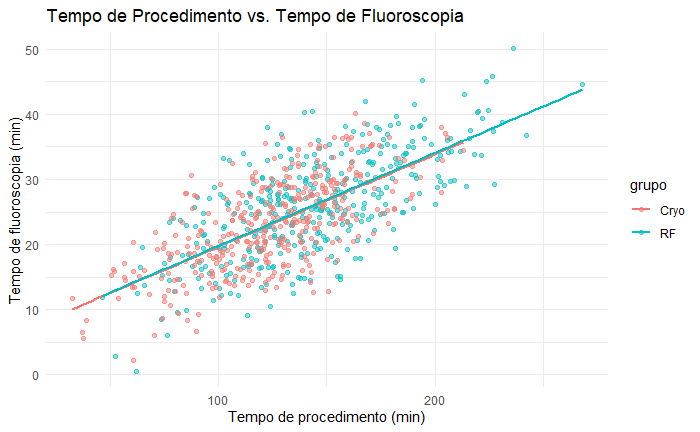
\includegraphics[width=0.8\textwidth]{img/quando.scatter.png}
    \caption{Relação entre tempo de procedimento e tempo de fluoroscopia.}
    \label{fig:scatter_plot}
\end{figure}

O gráfico sugere uma relação linear positiva: procedimentos mais longos
tendem a apresentar também maior tempo de fluoroscopia.

Podemos quantificar essa associação utilizando a correlação de Pearson:

\begin{code}[Código: correlação de Pearson]
resultado_cor <-
  cor.test(
    fire_ice$tempo_procedimento,
    fire_ice$tempo_fluoroscopia,
    method = "pearson"
  )

resultado_cor
\end{code}

O resultado da simulação é:

\begin{code}[Resultado da correlação]
	Pearson's product-moment correlation

data:  fire_ice$tempo_procedimento and fire_ice$tempo_fluoroscopia
t = 26.321, df = 748, p-value < 2.2e-16
alternative hypothesis: true correlation is not equal to 0
95 percent confidence interval:
 0.6543224 0.7288373
sample estimates:
      cor 
0.6934294 
\end{code}

O coeficiente de correlação estimado é:

\[
r = 0{,}693.
\]

O valor positivo indica que as duas variáveis tendem a aumentar juntas.
A magnitude do coeficiente indica uma associação linear positiva de
moderada a forte intensidade no contexto desta simulação.

O intervalo de confiança de $95\%$ para a correlação é aproximadamente:

\[
IC_{95\%} = (0{,}654,\;0{,}729).
\]

Isso indica que, sob as condições do modelo utilizado, os valores
compatíveis com os dados para a correlação populacional estão concentrados
em uma faixa positiva. O intervalo também fornece uma medida da incerteza
associada à estimativa de $r$.

O teste apresenta $p < 2{,}2\times10^{-16}$. Como esse valor é muito menor
que $0{,}05$, rejeitamos a hipótese nula de ausência de correlação linear.
Há, portanto, forte evidência estatística de uma associação linear entre o
tempo de procedimento e o tempo de fluoroscopia nesta simulação.

\begin{error}
\boxtitle{Correlação não é uma relação causal}

Mesmo quando $r$ é elevado e o valor de $p$ é muito pequeno, não podemos
concluir automaticamente que o aumento do tempo de procedimento cause o
aumento do tempo de fluoroscopia.

Neste exemplo, ambas as variáveis podem refletir a complexidade do
procedimento. Além disso, o tempo de fluoroscopia pode depender de fatores
como tecnologia disponível, experiência da equipe e estratégia utilizada.

Portanto, a correlação descreve uma associação observada nos dados simulados.
Ela não estabelece um mecanismo causal.
\end{error}

\begin{deepdive}
\boxtitle{Associação global pode esconder diferenças entre grupos}
Quando os dados pertencem a diferentes grupos, uma correlação calculada
considerando todos os participantes pode misturar fenômenos distintos.

Por exemplo, se RF e Cryo tiverem tempos médios de procedimento diferentes,
parte da associação global entre tempo de procedimento e fluoroscopia pode
estar relacionada simplesmente à diferença entre os grupos.

Por isso, em análises mais avançadas, pode ser útil:

\begin{itemize}
    \item colorir os pontos por grupo;
    \item calcular associações dentro de cada grupo;
    \item utilizar regressão para ajustar pelo grupo;
    \item investigar possíveis interações.
\end{itemize}

Esse problema é um exemplo de por que uma medida de associação isolada nem
sempre responde completamente à pergunta científica.
\end{deepdive}

\section{Como escolher o teste?}

A escolha do teste pode ser organizada a partir da pergunta científica e da
estrutura dos dados.

\begin{table}[htbp]
\centering
\caption{Guia inicial para escolha do procedimento estatístico}
\label{tab:escolha_teste}
\vspace{2mm}

\begin{tabular}{p{4.2cm} p{4.0cm} p{4.5cm}}
\toprule
\textbf{Pergunta} &
\textbf{Estrutura dos dados} &
\textbf{Procedimento possível} \\
\midrule

Comparar uma média com um valor de referência &
Uma variável quantitativa &
Teste-$t$ de uma amostra \\

Comparar duas médias independentes &
Variável quantitativa; dois grupos independentes &
Teste-$t$ de Welch \\

Comparar duas médias pareadas &
Variável quantitativa; duas medidas relacionadas &
Teste-$t$ pareado \\

Comparar três ou mais médias &
Variável quantitativa; grupos independentes &
ANOVA ou ANOVA de Welch \\

Comparar três ou mais grupos com condições inadequadas para ANOVA &
Dados ordinais ou distribuições muito assimétricas &
Kruskal--Wallis \\

Avaliar associação entre duas variáveis categóricas &
Tabela de contingência &
Qui-quadrado ou teste exato de Fisher \\

Avaliar associação linear entre duas variáveis quantitativas &
Duas variáveis quantitativas &
Correlação de Pearson \\

Avaliar associação monotônica sem pressupor linearidade &
Variáveis quantitativas ou ordinais &
Correlação de Spearman \\

\bottomrule
\end{tabular}
\end{table}

Essa tabela deve ser utilizada como um \textbf{ponto de partida}, e não como
uma árvore de decisão automática. O desenho do estudo, os pressupostos, a
estrutura dos dados e a medida de efeito de interesse podem exigir métodos
diferentes.

Por exemplo, dois grupos não implicam automaticamente um teste-$t$:
se a variável for categórica, uma tabela de contingência pode ser mais
apropriada; se as observações forem pareadas, o teste deve respeitar esse
pareamento; e se a pergunta envolver tempo até um evento, métodos de
sobrevivência podem ser necessários.


\end{document}